\documentclass[11pt]{article}

\usepackage{amsmath}
\usepackage{amssymb}
\usepackage{enumitem}
\usepackage[final]{graphicx}
\graphicspath{{./project_structure.pdf}}
\usepackage{xurl}
\usepackage{float}

\newcommand*{\courier}{\fontfamily{pcr}\selectfont}
\DeclareTextFontCommand{\code}{\courier}

\author{Erik Sturzenhecker, Felix Thiele}
\title{A Start to the formalization of Linear Algebra in ForTheL}

\date{\today}

\begin{document}
\maketitle

\newpage 
\setcounter{tocdepth}{10}
\tableofcontents


\newpage 
\section{Introduction}
\subsection{Naproche}
In this project we build a linear algebra library in ForTheL with Naproche. ForTheL, which stands for Formal Theory Language, is a language that comes close to human language. This reduces many of the initial hurdles people encounter in the formalization of mathematics. Naproche can not only interpret ForTheL code, but is also backed with a strong Automated Theorem Prover, to which we shall refer to as e-prover. This makes many Proofs in our library easier, since some trivial steps can be skipped. At the same time this comes with massive performance issues, since checking this small library is a comparably very time intensive task.

\subsection{Results}
Some of the results given in this library are:
\newline
The \textbf{definitions} of:
\begin{itemize}[nolistsep, noitemsep]
\item Groups, Rings, Fields
\item Vector spaces, Subspaces, Dual spaces
\item Homomorphisms, Endomorphisms, Automorphisms of vector spaces
\item Lists, Linear independence
\end{itemize}
And the \textbf{proofs} of:
\begin{itemize}[nolistsep, noitemsep]
\item A field is a vector space over itself.
\item The linear maps between $K$-vector spaces $V§$ and $W$ form a vector space Hom($K$,$V$,$W$).
\item If $f$ is linear, Ker($f$) is a subspace.
\item If $f$ is linear and Ker($f$) $=$ \{0\}, then $f$ is injective.
\item Any $K$-vector space $V$ can be embedded into the double dual space $(V^{*})^{*}$
\item The endomorphisms of a $K$-vector space $V$ form a ring End($K$,$V$).
\item The invertible elements of a ring form a multiplicative group.
\end{itemize}

\newpage



\section{The Lean File}
For inspiration on how to formalize linear algebra for a proof checker we looked into the file "vector\_space.lean" found under \url{https://github.com/kckennylau/Lean/blob/master/linear_algebra/vector_space.lean}. It is part of a small lean library by Kenny Lau containing formalizations of various mathematical topics. Lean is a theorem prover and a programming language based on dependent type theory. There is an extensive library of mathematical lean texts, the mathlib (\url{https://github.com/leanprover-community/mathlib}), maintained by lean users, which is used and build upon in vector\_space.lean.



\subsection{Mathematical Content}
The file vector\_space.lean covers the following definitions and statements of linear algebra:
\begin{itemize}
\item \code{field.to\_vector\_space}: Any field is a vector space over itself.
\item \code{sub\_vector\_space}: Definition of a vector subsace. Definition and proof of the vector space structure on it.
\item \code{linear\_space K V W}: Definition of the set of linear maps between two $K$-vector spaces $V$ and $W$. Easy proofs about linear maps.
\item \code{ker}: Definition of the kernel of a linear map. Some small proofs.
\item Definition and proof of the vector space structure on \code{linear\_space K V W}.
\item Definition of the dual vector space.
\item Definition and proof of the ring structure on \code{linear\_space K V V} by taking the function composition as multiplication.
\item \code{invertible K V}: Definition and proof of the (general linear) group structure on the invertible elements of \code{linear\_space K V V}
\end{itemize}
The respective notions are defined in the canonical way and the proofs are of course trivial from an algebraic standpoint. Thus, there is no need for huge lambda terms (which are otherwise are not uncommon in lean texts) and the code is fairly easy to understand.



\subsection{Characteristic Features}
- using the following notions from the mathilb: ... \\
- type classes: has\_add, has\_zero, etc. \\
- @[simp] (-> easy statements named above)\\
- ...



\subsection{Adjusting the Code}
The latest version of vector\_space.lean is from November 2017. Since then, it seems that the mathlib has developed to a point where it became incompatible with vector\_space.lean.
However, slight adjustments in the file made it work with the current version of the mathlib. This comprises the following changes:
\begin{itemize}
\item bla
\item blub
\end{itemize}

\newpage



\section{Formalization in ForTheL}
\subsection{Project Structure}
Giving the project a treelike structure with a file to each topic ensures increased readability and scalability. 
In contrast to having one large file building up mathematics, this enables us to pick what files need to be imported to each file. 
Our structure is depicted in the graph below.

\begin{figure}[h]
\begin{center}
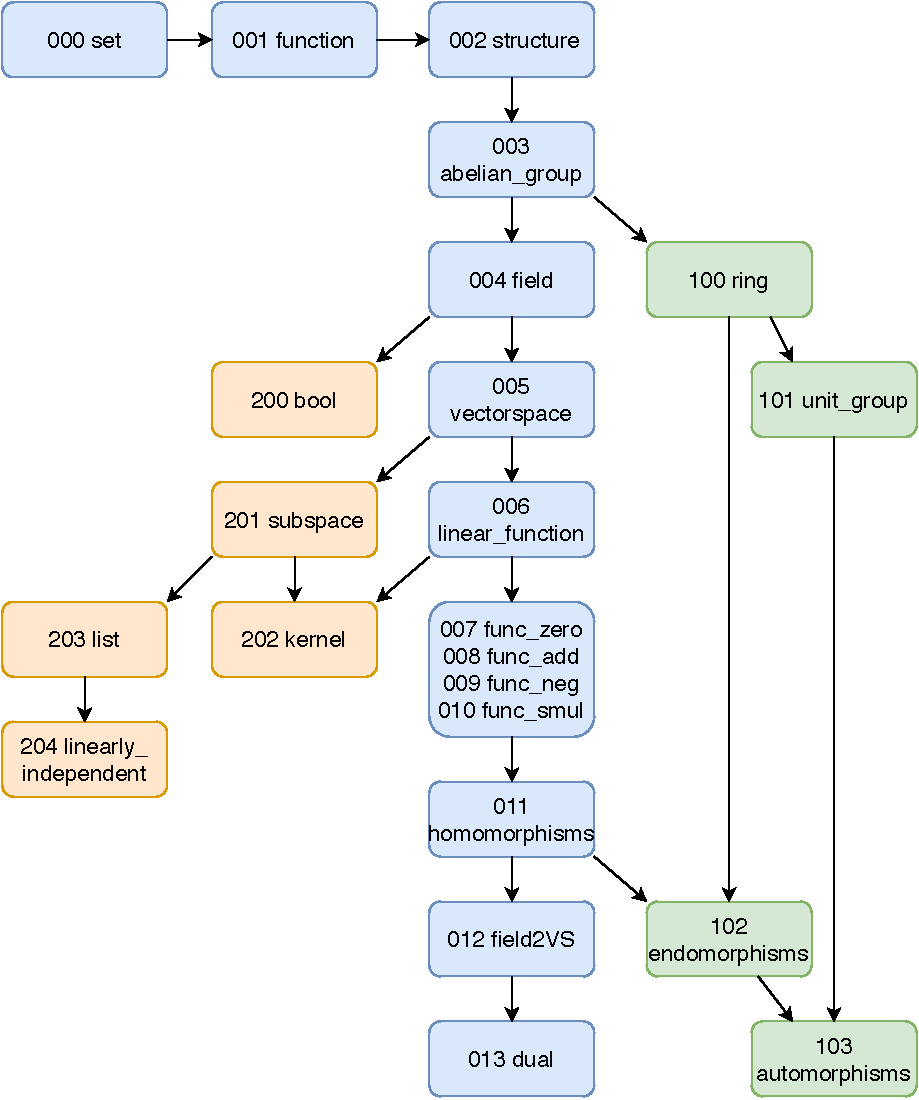
\includegraphics[scale=0.75]{./project_structure.pdf}
\end{center}
\end{figure}

\newpage

The e-prover is not fast enough to compile the entire library with all proofs in reasonable time. 
Instead, for every file we introduce two new files inserting "A\_" and "P\_" respectively in front of the file names. We insert "D\_" before our original file. This gives us an Axiom, Proof and Definition file. 
The Definition file holds all the definitions of the given topic. 
The Proof file holds the theorems and their proofs. The Axiom file holds all the statements of the Proof file in axiomatized form. 
The Proof and Axiom files only read their corresponding Definition file, while Definition files read the Axiom files of all the topics they are building upon. 
This ensures a fast compilation since we don't need to reprove proven statements. 
This file reading structure is depicted below.

\begin{figure}[h]
\begin{center}
\makebox[\linewidth][c]{
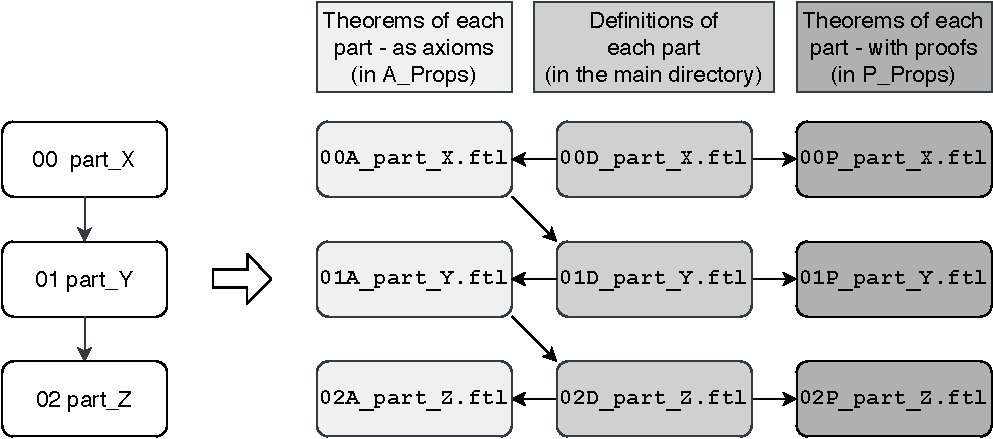
\includegraphics[scale=0.75]{./project_structure_explained.pdf}
}
\end{center}
\end{figure}

\subsection{The Implementation}

\subsubsection{Sets and Functions}

Our D\_ Set and D\_ Function files our kept very lightweight and only include key statements. This is due to both files being so close to the root node of the library tree. Adding more definitions will substantially slow down the e-prover in all following files.

\subsubsection{The structure object}
Many of the objects we examine in this library have a similar structure. For examples groups, fields, vector spaces and rings all have a carrier, a zero element, and an addition defined on them. We introduce the object structure in 002D\_ structure.ftl. 

\begin{figure}[H]
\begin{center}
\makebox[\linewidth][c]{
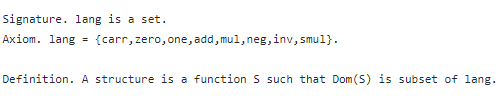
\includegraphics[scale=1]{./struc_def.png}
}
\end{center}
\end{figure}
We can now define a each of the linear algebra structures above as a structure with then necessary components of language in its domain. Now we define the following abbreviations:
\begin{figure}[H]
\centering
\begin{minipage}{.5\textwidth}
\makebox[\linewidth][c]{
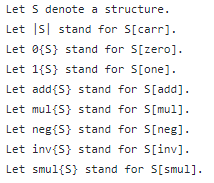
\includegraphics[scale=1]{./struc_simp1.png}
}
\end{minipage}%
\begin{minipage}{.5\textwidth}
\makebox[\linewidth][c]{
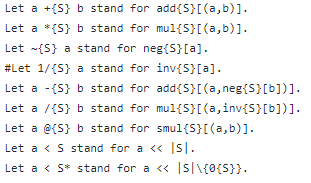
\includegraphics[scale=.8]{./struc_simp2.png}
}
\end{minipage}
\end{figure}

\subsubsection{Homomorphisms}

After the definition of various structures on sets we define homomorphisms. These require quite an extensive preparation which is done in the func\_ files, defining the zero, addition, negation, and scalar multiplication on Hom(K,V,W). These are split from the D\_ Homomorphism file because the corresponding P\_ files hold long proofs which become easier to read.

\subsubsection{Lists}

A list is defined as function from a set to a structure with a carrier and a zero element. The zero element ensures, that the list is not defined over an empty set of objects. 

\section{Comparison between Lean and Naproche}


\section{Next Steps in Naproche and ForTheL}

It seems like this project has hit somewhat of a ceiling in what naproche is capable of. 
Even small changes in beginning files can massively impact the check times.
While the main problem that needs to be addressed is a more efficient structuring and analysis of the cache, we propose the following ideas to improve the programming experience.

Firstly naproche needs an increased transparency in what the e-prover is doing. On the one hand the e-prover is a huge blessing, simplifying many steps. On the other hand it is the source of many problems, since the programmer can not guess where the e-prover gets stuck. Also the e-prover will often take longer or even cant compile working code, if it is copied to a later part of the file. This is due to the increased breadth of the internal search tree. To counter these effects, while keeping the luxury of an assisting e-prover, we suggest the e-prover return the proofs of each statement, which can then be either pasted into the code or be saved in a separate file. This decoupling of the e-prover to the checking process will not only save time, but also guarantee more stability.

ForTheL needs a Code Sectioning functionality. This would not only improve code transparency but also speed up checking times. At the moment the e-prover can only be restricted by (by theorem) commands. Introducing code sections will allow broader restrictions.

\end{document}

